\documentclass[12pt]{article}
\usepackage[utf8]{inputenc}
\usepackage{enumitem}
\usepackage{amscd,amsfonts,amsmath,amssymb,amsthm,amsxtra,amstext,mathtools,
	latexsym,bbm,enumitem,indentfirst,bm,emptypage,color,pifont,float}
\usepackage[titletoc]{appendix}
\usepackage[nottoc,notlot,notlof]{tocbibind}



% set margins for double-sided printing
\usepackage[letterpaper,total={5.5in,9in}, top=1.0in, inner=1.5in, outer=1.0in,bottom=1.0in,,headheight=0pt,headsep=0pt,centering]{geometry}

% Title Page
\title{MOVER: Multi-Objective Optimization for VErsatile Materials Research}
\author{Conrrad Giresse Tetsassi Feugmo}
\linespread{1.3}

\begin{document}
\maketitle



\section{introduction}

MOVER: Multi-Objective Optimization for VErsatile Materials Research is an  implementation of Multi-objective Optimization for Materials Discovery via AdaptiveDesign (Gopakumar, A.M., Balachandran, P.V., Xue, D. et al. Multi-objective Optimization for Materials Discovery via Adaptive Design. Sci Rep 8, 3738 (2018). https://doi.org/10.1038/s41598-018-21936-)



\section{single objective}



	For a single objective, given a material property $y$ dependent on features, also called descriptors, $x$, machine learning allows us to estimate a function $f(x)$ from the training data, such that $y=f(x)$. However, in order to minimize the number of new materials that need to be experimentally tested, say, to find the material with the smallest $y$, we can choose a newly calculated design point $y(x^{N+1})$ representing an improvement over the current best design, $\min f(x)=\min[f_1(x_1), f_2(x_2),\dots, f_N(x_N)]$, using $P[I]$ and $E[I]$, the probability and expected value of improvement.

	The improvement $I$ is given by
	\begin{align*}
		I &= \min f(x) - y(x^{N+1})
	\end{align*}

	The probability of improvement $P[I]$ is given by
	\begin{align*}
		P[I] &= \Phi\left(\frac{\min f(x) - \mu(x^{N+1})}{\sigma(x^{N+1})}\right)
	\end{align*}
	where $\mu$ is the mean and $\sigma$ is the standard deviation. $\Phi$ is the cumulative distribution function of the Gaussian integrands, and we have assumed that the new points are distributed according to a Gaussian distribution.

	The expected improvement $E[I]$ is given by
	\begin{align*}
		E[I] &= \left(\min f(x) - y(x^{N+1})\right) + \Phi\left(\frac{\min f(x) - \mu(x^{N+1})}{\sigma(x^{N+1})}\right) \
		+ \sigma\phi\left(\frac{\min f(x) - \mu(x^{N+1})}{\sigma(x^{N+1})}\right)
	\end{align*}
	where $\phi$ is the Gaussian probability density function.

	\section{two-objective optimization problem}


	\begin{figure}[!h]
		\centering
		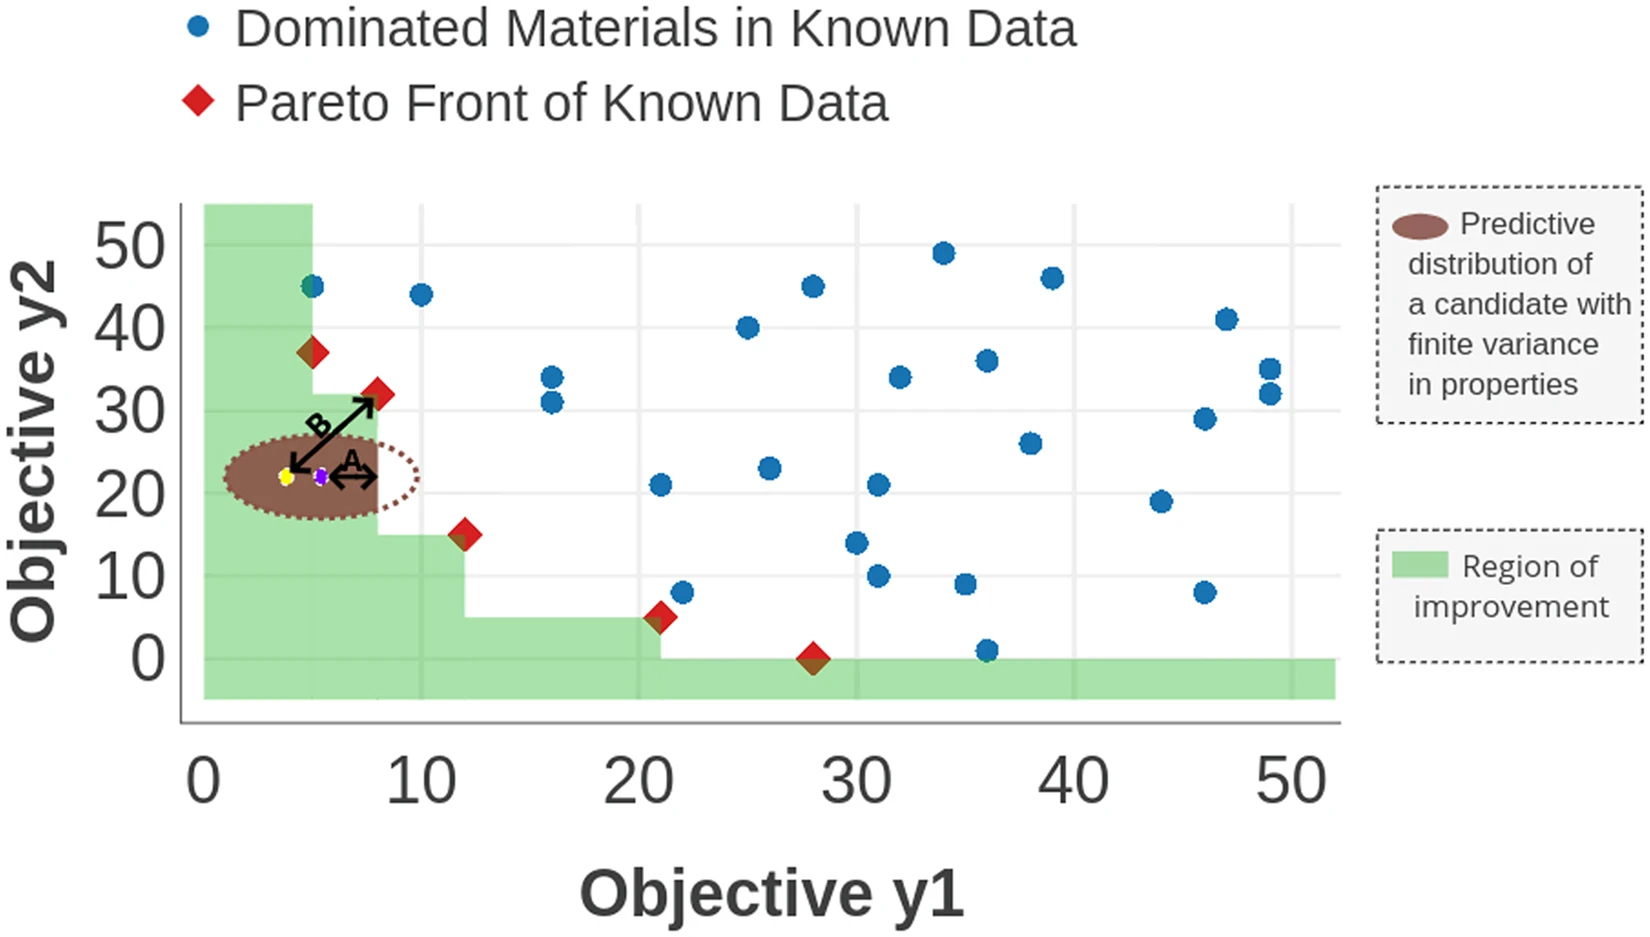
\includegraphics[width=0.7\linewidth]{PF.jpg}
		\caption{}
		\label{fig:pf}
	\end{figure}

	Our focus here is on the application to materials of the two-objective optimization problem.
	\begin{align*}
	\text{Probability of Improvement}\; P[I]=\int_S \phi(y_1, y_2) \mathrm{d}y_1\mathrm{d}y_2,
		\end{align*} where $y_1$ and $y_2$ are the objectives and $\phi(y_1, y_2)$ is the uncorrelated
	Gaussian probability distribution function formed from the mean and
	variance of $y_1$ and $y_2$ distributions with $\phi(y_1, y_2) = \phi(y_1) \phi(y_2)$.
	We have therefore assumed a Gaussian distribution for the predicted
	values with a mean and variance.

	Similarly, the equivalent two objective expected improvement $E[I(x)]$
	is the first moment of $I$ of the joint probability distribution $\phi(y_1, y_2)$.

	Geometrically, we can calculate the Expected Improvement $E[I(x)] = P[I(x)]L$ in
	two ways depending on how the ``length'' $L$ is evaluated: using the

\begin{enumerate}[label=(\alph*)]
		\item  Centroid approach to EI, referred to as EI-Centroid: $E[I(x)] = P[I(x)]L$, where

		$L=\sqrt{[Y_1(x)-y_1(x)]^2+[Y_2(x)-y_2(x)]^2}$, the distance between the centroid $(Y_1(x), Y_2(x))$ at the candidate
		data point, $x$, and closest point on the subPareto front, $(y_1(x), y_2(x))$.
		The centroid of the probability distribution for the candidate point is calculated using

		\begin{align*}
			Y_1(x)&=\frac{\int_S y_1\phi(y_1, y_2)\mathrm{d}y_1\mathrm{d}y_2}{P[I]}\\
			Y_2(x)&=\frac{\int_S y_2\phi(y_1, y_2)\mathrm{d}y_1\mathrm{d}y_2}{P[I]}\\
		\end{align*}


	\item Maximin approach to EI, referred to as EI-maximin:
	Let the mean predicted values for a candidate material be $(\mu_1, \mu_2)$.
	Then we define the distance $d_{maximin} = \max_i(\min(p_{i1}-\mu_1, p_{i2}-\mu_2), 0)$, where $P_i=(p_{i1}, p_{i2})$ and $P_i \in PF$.
	The maximin Expected Improvement is then $EI_{maximin}=d_{maximin} \times P[I(x)]$.

\end{enumerate}

	Thus, for each candidate point in the region of improvement,
	EI-Centroid is calculated by taking the product of $P[I]$ with the minimum distance between
	points on the known sub pareto front and centroid of the probability distribution within the region of improvement.
	The candidate point with the largest EI-Centroid is then the choice for the next measurement.
	EI-maximin is the product of $P[I]$ and the maximum of the minimum distance of either of the means $(\mu_1, \mu_2)$
	of a particular candidate point from individual sub Pareto front points $p_i$.
	The former considers improvement over the properties $y_1$, $y_2$ combined,
	whereas EI-maximin considers each property separately, takes the one which is smaller from a particular subPareto point,
	and then maximizes that amongst all the subPareto points.

	We will implemented both EI-Centroid and EI-maximin strategies and also compared them against:

\begin{enumerate}[label=(\roman*)]
		\item  Random selection,
		\item  Pure exploitation using only the mean values of predictions from a machine-learned model, and
		\item  Pure exploration, where the  selection is based on the magnitude of the variance for candidate points in the region of improvement.
\end{enumerate}


%	The results showed that both EI-Centroid and EI-maximin outperformed the other strategies in terms of identifying points that modify the sub Pareto front the most. EI-Centroid performs better when the sub Pareto front is nearly linear, while EI-maximin performs better when the sub Pareto front has a more complex shape.
%
%	In summary, the two-objective optimization problem in materials can be approached using the Probability of Improvement and Expected Improvement criteria. The EI-Centroid and EI-maximin strategies can be used to select candidate points for measurement to modify the sub Pareto front, outperforming other strategies such as random selection, pure exploitation, and pure exploration.


\end{document}
